\begin{alist}
\item Η ανίσωση $\dfrac{\omega^2 - 1}{\omega - 3} > 0$ με $\omega \ne 3$ είναι ισοδύναμη με την $(\omega^2 - 1)(\omega - 3) > 0$. \\
Το πρόσημο του $(\omega^2 - 1)(\omega - 3)$ φαίνεται στον παρακάτω πίνακα.

\begin{center}
\begin{tikzpicture}
\tkzTabInit[lgt=4, espcl=1.5]
  {$\omega$ /1, $\omega-3$ /1.5, $\omega^2 - 1$ /1.5, $(\omega-3)(\omega^2-1)$ /2}
  {$-\infty$, $-1$, $1$, $3$, $+\infty$}
\tkzTabLine{ , -, t, -, t, -, z, +, }
\tkzTabLine{ , +, z, -, z, +, t, +, }
\tkzTabLine{ , -, z, +, z, -, z, +, }
\end{tikzpicture}
\end{center}

Συνεπώς η ανίσωση $\dfrac{\omega^2 - 1}{\omega - 3} > 0$ αληθεύει για κάθε $\omega \in (-1, 1) \cup (3, +\infty)$.

\item Η παράσταση $A$ ορίζεται για κάθε πραγματική τιμή του $x$ για την οποία ισχύει $\dfrac{e^{2x} - 1}{e^x - 3} > 0$. Αν θέσουμε $e^x = \omega$ η ανίσωση $\dfrac{e^{2x} - 1}{e^x - 3} > 0$ γίνεται $\dfrac{\omega^2 - 1}{\omega - 3} > 0$ που όπως δείξαμε στο α) αληθεύει για $\omega \in (-1, 1) \cup (3, +\infty)$. \\
Συνεπώς θα πρέπει $-1 < \omega < 1 \Leftrightarrow -1 < e^x < 1 \Leftrightarrow x < 0$ ή $\omega > 3 \Leftrightarrow e^x > 3 \Leftrightarrow x > \ln 3$. \\
Τελικά η παράσταση $A$ ορίζεται για κάθε $x \in (-\infty, 0) \cup (\ln 3, +\infty)$.

\item Η εξίσωση $A = -\ln 3$ ορίζεται για κάθε $x \in (-\infty, 0) \cup (\ln 3, +\infty)$ και γίνεται ισοδύναμα
\begin{align*}
\ln\left( \frac{e^{2x} - 1}{e^x - 3} \right) &= \ln 3^{-1} \Leftrightarrow \\
\frac{e^{2x} - 1}{e^x - 3} &= \frac{1}{3} \Leftrightarrow \\
3e^{2x} - 3 &= e^x - 3 \Leftrightarrow \\
3e^{2x} - e^x &= 0 \Leftrightarrow \\
e^x(3e^x - 1) &= 0 \overset{e^x \ne 0}{\Leftrightarrow} \\
3e^x - 1 &= 0 \Leftrightarrow \\
e^x &= \frac{1}{3} \Leftrightarrow \\
x &= \ln\frac{1}{3}
\end{align*}
και επειδή $\dfrac{1}{3} < 1 \Leftrightarrow \ln\dfrac{1}{3} < 0$ η λύση $x = \ln\dfrac{1}{3}$ είναι δεκτή.
\end{alist}
